%%%%%%%%%%%%%%%%%%%%%%%%%%%%%% -*- Mode: Latex -*- %%%%%%%%%%%%%%%%%%%%%%%%%%%%
%% nsf.tex         : 2009 CPATH Proposal
%% Author          : Philip Johnson
%% Created On      : Tue Mar 31 11:16:58 2009
%% Last Modified By: Philip Johnson
%% Last Modified On: Wed Dec  2 13:57:02 2009
%%%%%%%%%%%%%%%%%%%%%%%%%%%%%%%%%%%%%%%%%%%%%%%%%%%%%%%%%%%%%%%%%%%%%%%%%%%%%%%
%%   Copyright (C) 2009 
%%%%%%%%%%%%%%%%%%%%%%%%%%%%%%%%%%%%%%%%%%%%%%%%%%%%%%%%%%%%%%%%%%%%%%%%%%%%%%%
%% 
 
\documentclass[11pt]{article}
\usepackage[final]{graphicx}

%% Make subsubsections numbered and included in ToC
\setcounter{secnumdepth}{3}
\setcounter{tocdepth}{3}

%% URLs
\usepackage{url}
\usepackage[colorlinks, bookmarks=true]{hyperref}

%% Define a new 'smallurl' style for the package that will use a smaller font.
\makeatletter
\def\url@smallurlstyle{%
  \@ifundefined{selectfont}{\def\UrlFont{\sf}}{\def\UrlFont{\small\ttfamily}}}
\makeatother
%% Now actually use the newly defined style.
\urlstyle{smallurl}

%% CO2 
\usepackage{xspace}
\newcommand{\COtwo}{CO\ensuremath{_2}\xspace}

%% Make margins less ridiculous
\usepackage{fullpage}


%% Since I'm using the LaTeX Makefile that uses dvips, I need this
%% package to make URLs break nicely
\usepackage{breakurl}

\begin{document}
\title{Human centered information integration\\ for the Smart Grid}

\author{Philip M. Johnson \\
      Collaborative Software Development Laboratory \\
      Department of Information and Computer Sciences \\
      University of Hawai'i,  Honolulu, HI 96822 \\
      johnson@hawaii.edu
}

\maketitle
\tableofcontents
\newpage

%%%%%%%%%%%%%%%%%%%%%%%%%%%%%% -*- Mode: Latex -*- %%%%%%%%%%%%%%%%%%%%%%%%%%%%
%% project-techreport.tex -- 
%% Author          : Philip Johnson
%% Created On      : Tue Mar 31 11:44:58 2009
%% Last Modified By: Philip Johnson
%% Last Modified On: Thu Dec 10 10:08:30 2009
%% RCS: $Id$
%%%%%%%%%%%%%%%%%%%%%%%%%%%%%%%%%%%%%%%%%%%%%%%%%%%%%%%%%%%%%%%%%%%%%%%%%%%%%%%
%%   Copyright (C) 2009 
%%%%%%%%%%%%%%%%%%%%%%%%%%%%%%%%%%%%%%%%%%%%%%%%%%%%%%%%%%%%%%%%%%%%%%%%%%%%%%%
%% 

\section{Introduction}

Development of the ``Smart Grid'', a modernized power infrastructure, is
one of the key technological challenges facing the United States at the
dawn of the 21st century. According to the Department of Energy, the smart
grid should: (1) Enable active participation by consumers by providing
choices and incentives to modify electricity purchasing patterns and
behavior; (2) Accommodate all generation and storage options, including
wind and solar power.  (3) Enable new products, services, and markets
through a flexible market providing cost-benefit tradeoffs to consumers and
market participants; (4) Provide reliable power that is relatively
interruption-free; (5) Optimize asset utilization and maximize operational
efficiency; (6) Provide the ability to self-heal by anticipating and
responding to system disturbances; (7) Resist attacks on physical
infrastructure by natural disasters and attacks on cyber-structure by
malware and hackers \cite{NETL:GridCharacteristics}.

In October, 2009, the government awarded approximately \$3.4 billion in
federal stimulus money to approximately 100 organizations in 49 states to
support Smart Grid development.  While substantial, this investment is
almost totally focused on low-level infrastructure including meters,
communication networks, and phasor measurement units.  By analogy to the
Internet, this investment is similar to upgrading a copper wire network to
fiber optic cable, along with installation of high performance routers and
name servers.  Such infrastructure is a necessary requirement for
high-level Internet services such as the World Wide Web, but does
relatively little to determine the nature of those services.

The Smart Grid will produce and consume information about electricity as
well as electricity itself, thus forming a specialized kind of Internet. At
the current time, it is not clear what ecosystem of higher-level services
should be developed to best communicate, analyze and interpret this
low-level electrical data to consumers.  (By ``consumers'', we mean all of
the various customers of utilities: both individuals and businesses
alike. )

One reason why there is little clarity about consumer-facing information
services in the Smart Grid is the nature of the current grid, which (from a
consumer point of view) is a classic ``black box'' technology.  For almost
100 years, customers have plugged appliances into electrical outlets and
expected them to ``just work''.  Put another way, the U.S. power industry
has operated for a century under the assumption that consumers should have
{\em reliable} access to a virtually {\em unlimited} amount of {\em high
  quality} electricity.  Traditionally, residential consumers have been
given extremely little information about electricity beyond a monthly bill.

This ``Electricity As Black Box'' paradigm requires electricity to be cheap,
reliable, and unlimited, but those days appear to be ending for a number of
reasons.  First, the heavy reliance on fossil fuels for power generation is
not sustainable: most economists agree that ``peak oil'' has either already
occurred or will occur in the next two decades. After that point, oil
supply will decrease and prices will increase.  Second, fossil fuels
generate green house gases that contribute to climate change, and so there
is a need to move to less carbon intensive energy sources such as solar,
wind, wave, and geothermal.  Third, reliance on fossil fuels creates a
variety of political problems.

Could the Electricity As Black Box paradigm be maintained by simply
replacing fossil fuel by renewable energy sources? Unfortunately,
unlike fossil-fuel based power generation, most renewable energy sources
depend upon generally unpredictable environmental
factors.  As a result, simply adding a solar panel to every rooftop and
tying them into the grid would do more harm than good at present.
This is because grid stability requires energy production to equal energy demand
on a second to second basis, and utilities generally do not have a way to
monitor and balance a grid that incorporates high levels of widespread,
variable, and distributed generation. 

Another candidate for preserving the Electricity As Black Box paradigm
is ``demand-response'' technology.  With demand response,
utilities obtain control over major appliances in the home such as the hot
water heater and the heating/cooling system. At peak times, utilities can
shut off the water heater or change thermostat settings in order to reduce
the load on the grid.  While demand response can be effective and is
already deployed in some commercial settings, it is not clear that
consumers will universally accept utility-based control of their home
systems.  For example, a recent study of Boulder residents found that
approximately 50\% of those surveyed would not want demand-response
installed in their house \cite{Farhar09}.

Even if electricity could remain a black box to consumers, there is
compelling evidence suggesting that it should not.  According to the July
2009 report ``Unlocking energy efficiency in the U.S. Economy''
\cite{Granade09}, there is the potential to reduce annual
non-transportation energy consumption by roughly 23 percent by 2020,
eliminating more than \$1.2 trillion in waste.  Such a reduction in energy
use would result in abatement of 1.1 gigatons of greenhouse gas emissions
annually. ``Unlocking'' this untapped potential requires, in part, improved
access by consumers to energy information, along with changes in behavior
based on this information that produce the desired efficiencies.

The view that electricity cannot and should not remain a black box to
consumers motivates the central question of this research: just what kind of
``white box'' should it become?  More specifically, {\em What kinds of
  information, provided in what ways and at what times, enables consumers
  to make positive, sustained changes to their energy consumption
  behaviors?}

In this research, we propose to develop technologies and experimental
methods that support more efficient and effective scientific study of the
ways in which access to information about energy usage impacts on consumer
behavior.  Our work will build upon current energy user interface successes
and failures; leverage emerging Smart Grid standards; incorporate open
source and component-oriented development techniques; and respect findings
from behavioral research. Based upon current research and our prior
experience, we will implement a novel open source framework for energy data
collection, storage, analysis, and presentation called WattBlocks, along
with a novel social networking application for energy behavioral change
called eSpheres.  

To evaluate these innovations, we will carry out a series of case studies:
one focusing on university campus dormitory competitions and one focusing
on community residential energy challenges. We choose these two domains
because they are of growing popularity and have contrasting demographic
characteristics.  Our studies will help establish standardized technology
and methodological support that foster replication, meta-analysis of data,
and quicker convergence to scientifically-based understanding of energy
information needs and behaviors in the Smart Grid.

The anticipated contributions of this research will include: (1) outcome
data from our two case studies that provide new insight into requirements
for Smart Grid information services; (2) replicable methods for inquiry
into Smart Grid technologies and their impact on consumers; (3) open
source technologies to facilitate scientific experimentation on the Smart
Grid; and (4) a unique approach to organizing energy information and
interaction as nested ``energy community spheres'', which attempts to solve
problems with context and provide greater opportunities for engagement and
behavioral change.

The remainder of this proposal is organized as follows.  Section
\ref{sec:related-work} overviews research and technologies that serve as a
basis for our approach.  Section \ref{sec:methodology} presents our proposed
experimental approach.  Section \ref{sec:merit} discusses the intellectual
merit and broader impact of this research. 

\section{Related work}
\label{sec:related-work}

Our proposed research combines insights from behavioral research on energy
efficiency along with prior approaches to energy data collection and analysis.

\subsection{Energy and behavior}

For utilities that are attempting to move beyond the Electricity As Black
Box paradigm, the traditional approach involves providing financial
incentives to consumers to adopt energy efficient devices and products.
Adoption can occur when a consumer buys something new (like a new house or
light bulb) or when they replace an existing product.  Energy efficiency
improvements come from changing the efficiency of the technology consumers
are using, not from changing their use of that technology.  This approach
has been termed the Physical, Technical, and Economic Model (PTEM)
\cite{Lutzenhiser93}.  PTEM takes an engineering-centric approach to energy
efficiency, assuming that energy use is only affected by new technology,
whose adoption is only affected by price subsidies. As the approach adopted
by most utilities, it is the reason why the vast majority of residential
energy efficiency programs rely on product rebates to incentivize purchases
of energy efficient products and services. PTEM is an attractive model
because it doesn't require consumers to change the way they use energy, and
it doesn't require any effort to ensure that any change in behavior
persists.

Unfortunately, a variety of research indicates that human behavior with
respect to energy cannot be modeled simply in terms of cost-effectiveness,
as is assumed by the PTEM model.  Granade \cite{Granade09} shows that the
PTEM model fails on a large scale, as almost a quarter of U.S. energy
consumption would not exist if consumers actually responded to all
cost-effective energy saving measures.

Problems with PTEM can also be demonstrated on a smaller scale.  For
example, Geller \cite{Geller81} performed an experiment in which 40
consumers attended a three hour workshop on energy conservation.  A pre and
post workshop questionnaire determined that all participants gained greater
awareness of energy issues, more appreciation for what could be done in
their homes to reduce energy use and save money, and a willingness to
implement the changes that were advocated in the workshop. However, a one
month followup indicated very little actual change in behavior. One person
lowered the temperature on the hot water heater. Two additional people had
installed insulating blankets around their hot water heaters, but they had
already done this before the workshop. Finally, eight people installed
low-flow shower heads---after all 40 participants had been given the
low-flow shower heads at the workshop.

A final issue with the PTEM model is that it fails to explain consumers who
reduce their energy usage even when they do not gain any financial benefit
from doing so.  For example, an increasingly popular and successful
university activity is the Dormitory Energy Challenge, in which residents
of one or more dormitories compete to reduce their dorm's energy
consumption (even though their housing bill will not change as a result).
Challenges at Brandeis University, Carleton College, Harvard University,
MIT, Mount Holyoke College, Ohio University, and Williams College have
reported energy savings, generally in the range of 7\% to 16\%.  John
Peterson leads what is perhaps the longest running dorm energy challenge
research project at Oberlin College \cite{Peterson07,Peterson07a}.  He is
currently investigating not only ambient devices, but also expanding to
other resources beyond energy, such as water.

Based upon these and other studies, a more nuanced model is beginning to
emerge in which at least the following factors appear to influence energy
behavior.  First, to influence behavior, provide {\em personalized
  information} that reflects the consumer's unique circumstances.  For
example, a dorm resident will not respond well to energy tips involving
improved insulation.  Second, provide both {\em general and specific
  commitments}, especially when they can be tied to a broader issue. For
example, pledging to use a clothesline rather than a dryer because it
reduces green house gas emissions.  Third, provide {\em achievable goals}
that can be objectively measured.  An example might be to reduce energy
consumption by 10\% over the previous month.  Fourth, elicit {\em social
  reinforcement} which can be manifested in both overt and subtle ways.  For
example, in dorm settings, as more and more residents publically
participate, it implicitly becomes ``the thing to do''.  Fifth, provide
{\em constant and contextual feedback} which helps verify progress toward
goals and can reinvigorate commitments, as long as the feedback is provided
in the right way at the right time.  Sixth, {\em financial incentives} can
be a powerful motivator for energy conservation when paired with one or
more of these other factors.

The first research on behavioral approaches to modifying energy consumption
occurred during the first energy crisis of the late 1970s. Becker found
significant effects from combining energy saving goals and feedback
\cite{Becker78} .  Households committed to goals of either 2 percent or 20
percent energy savings, and then a subset of each group were given feedback
on how well they were doing. The group that received the higher goal and
feedback reduced their actual usage by an average of 15 percent, while the
groups that received either the higher goal or the feedback reduced energy
use by about 5 percent.  Similarly, Houwelingen found that feedback and
goal setting produced a reduction of 12\% in energy use, and that usage
returned to prior levels if the feedback device was removed
\cite{Houwelingen89}.

Vollink and Meertens combined information, feedback, and goal-setting to
produce very significant savings: 23 percent natural gas reductions, 15
percent electricity reductions and 18 percent less water \cite{Vollink99}.
Staats et al. developed a program involving ``Eco-Teams'' of 6-10 people
who met once a month to discuss energy conservation and related
topics. These teams achieved sustained energy reductions averaging 7.5\% over
three years by combining information, social reinforcement, and feedback
\cite{Staats04}.

Faruqui et al \cite{Faruqui09} performed a review of over a dozen pilot projects
performed by utilities involving in-home displays which provide near-real
time feedback.  The authors found evidence that the introduction of this
single motivational factor (feedback) did appear to influence behavior:
consumers self-reported average reductions of around 7\%.   When paired with an
additional motivator (cost savings), average reductions increased to around
15\%.  However, these studies do not provide much evidence concerning the
sustainability of the changes; it could be that consumers will eventually
acclimate to the real-time display and cease conservation behaviors. 

As noted by Darby \cite{Darby06}, feedback is a necessary but
not always sufficient condition for savings and awareness among
consumers. Darby maintains that  the condition of housing, personal contact
with a trustworthy advisor when needed, and the availability of technology, 
training, and social infrastructure for learning may also be required 
in order for long-term change to occur.  

Recent behavioral research  has made great strides in moving beyond the
traditional PTEM model and has started to reveal important factors in
changing consumer energy behavior. But the connection to the Smart Grid is
still tenuous, the most appropriate motivational factors to apply to
particular circumstances is still unknown, and the effective use of modern
information technology such as social networks is almost virtually
unexplored.   The next section focuses on information technology. 

\subsection{Energy data interfaces}

Unfortunately, many of the meters currently designed for the Smart Grid
(such as those designed by Enel and Telvent) do not even provide a
consumer-facing interface; instead, they simply report on electrical usage
directly to the utility.  This simplifies billing operations for the
utility, but provides no direct feedback to the consumer.

Whether using a Smart Grid meter with a consumer-facing interface, or a
home energy monitoring system, the most common form of interface to energy
data provides a simple line chart or histogram of energy usage over various
time intervals: minutes, hours, days, or weeks.  Examples include home
energy monitoring systems such as the TED 5000; Google's PowerMeter
application, and building information management systems such as those by
Obvius, Lucid Design Group, Small Energy Group, and AgileWaves. In some
cases, these systems can display energy usage in alternative units, such as
carbon emitted or cost.  Figure \ref{fig:LucidDesignGroup} shows a
representative interface from Lucid Design Group.

\begin{floatingfigure}[l]{3.25in}
  \center
  \includegraphics[width=0.5\textwidth]{luciddesigngroup.3.eps}
  \caption{\em \small Building Dashboard, LucidDesignGroup}
  \label{fig:LucidDesignGroup}
\end{floatingfigure} 


At the utility-level, there are attempts to show grid-level information
through sites such as Ecotricity \cite{Ecotricity} or CurrentEnergy
\cite{CurrentEnergy}.  While most adhere to the standard line chart style
of visualization, the Ecotricity site also provides an interpretation of
the data with a stoplight that shows red, yellow, or green depending upon
the amount of carbon being produced by the grid at the current time.  The
goal of the stop light is to provide consumers with the information
necessary to enable them to shift energy-intensive tasks (such as running
their dryer) away from times when carbon intensity is high.

An emerging approach to energy interfaces is ``Eco-Visualization'',
defined by Pierce as ``Any kind of interactive device targetted at
revealing energy use in order to promote more sustainable behaviors or
foster postive attitudes towards sustainable practices \cite{Pierce08}.''
The seminal eco-visualization is called ``7000 oaks and counting'' by
Tiffany Holmes \cite{Holmes07}.  In the visualization, rings of spinning
oak trees represent carbon loads for a given environment from a single
building to a city.  If the loads are low, the rings are composed of green
trees. As loads increase, trees are removed and replaced by appliances such
as light bulbs or refridgerators.  Another eco-visualization involves a
virtual polar bear floating on an ice floe. The ice floe grows when users
commit to environmental actions and decreases when users choose not to
commit to change \cite{Dillahunt08}.

There is also movement toward interfaces apart from traditional websites.
For example, Lucid Design Group and Oberlin College are planning to
experiment with the use of ambient orbs to indicate energy consumption
\cite{Peterson09}.  The StepGreen system attempts to leverage social
networking sites like FaceBook and MySpace to enable sustainable behavior
\cite{Mankoff07}.

Not all interfaces focus exclusively on energy data.  For example, the
Energy Pledge prototype was designed for public display of personal
commitments \cite{Pierce09}.  The StepGreen system also provides a display
of commitments.  

While these various interface directions are promising and many have
yielded positive initial results, they do not address some issues and leave
other questions unanswered. First, it is often not clear whether or not and
how a given technology could be re-used in a new context.  Many of the
systems are either stand-alone (such as Stepgreen) or appear highly
customized to a specific context (Oberlin's Campus Resource
System). Second, there tends to be a single focus to the interface: either
very specific (one's dorm), or very general (the overall grid).  

\subsection{Energy data design issues}

The growing popularity of energy data related information systems is
heartening, but also demonstrates that much more can be done. 

First, the current state of consumer-facing energy information technology
is reminiscent of web site technology prior to the development of content
management systems such as Plone or Drupal, where lack of infrastructure
meant that web site developers were repeatedly re-implementing the same
basic functionality for navigation, page templates, file uploads, and so
forth, or paying a commercial provider to do it for them.  There are no
open source energy information technologies equivalent to Plone that
enables, for example, a university to quickly build a new dorm energy
challenge system from generic components.  No current system has an
architecture that facilitates ``mashups'' or ``plugins'', such that a
developer could quickly build an interface to a new technology such as
Google Wave, or integrate a new approach to commitments. This slows the
pace of innovation and progress toward understanding how to best improve
energy behaviors.

Second, energy information technologies are not designed to be amenable to
scientific research.  To gauge the effectiveness of an information
capability, it is helpful to gain a detailed understanding of how it is
accessed, by whom, and under what circumstances, and how that connects
to outcomes.  Such instrumentation support appears to be largely lacking
from current approaches.

In addition to instrumentation, it is often scientifically useful to
support treatments: in other words, providing different forms of
information to different populations of users in order to gain insight into
the effect of a treatment upon an outcome of interest. For example, one way
to assess the effect of commitments on energy conservation would be to
provide a ``Pledge Wall'' to only half the floors in a dorm, then use a
combination of qualitative (post-study interviews) and quantitative (actual
changes in energy) to assess the impact of that behavioral
treatment. Current systems take an ``all or nothing'' approach to
features. 

Finally, no current information system spans energy information from the ``micro''
(i.e. single building) to the ``macro'' (i.e. utility-level grid).  For
example, current in-home energy meters provide no insight into the carbon
intensity of the grid currently supplying the power to the home appliances.
Grid-level information systems like Ecotricity or CurrentEnergy do not
allow drill down to individual cities or homes.  As a result, interesting
opportunities to influence energy behavior are lost, such as a commitment
like ``I will use my dorm's dryer only when the carbon intensity of the grid is low.''

\section{Gaining insight into Smart Grid information needs}
\label{sec:methodology}

To provide better insight into the requirements of the Smart Grid for
support of sustained, positive behavioral change, this research will
involve a combination of  technology development and case studies.

\subsection{Technology Development}

\subsubsection{WattBlocks}

As we note above, current energy information systems tend to be closed,
either due to proprietary licensing or due to an architecture that limits
extensibility and reuse.  During the past ten years, we have developed
expertise in the design, implementation, and evaluation of open source,
extensible architectures through the Hackystat Project
\cite{csdl2-06-06,csdl2-09-02,csdl2-09-07,csdl2-09-01}.

Hackystat is an open source, scalable, extensible framework for collection,
analysis, interpretation, and dissemination of software engineering process
and product data.  It has been under continuous development for almost a
decade with contributions from over 30 software developers and usage by
thousands of people in academic, government, and industrial
organizations. The current version of Hackystat comprises over 250,000
lines of code, written in a variety of languages, and spread over more than
40 interdependent software systems.  Hackystat implements a
service-oriented architecture, where software engineering data is first
gathered by ``sensors'' and sent to a low-level repository for storage.
The data is abstracted by one or more middleware analysis components, and
finally presented to the user through one or more user interface
components.  Hackystat components typically implement a RESTful API, and
user interface components have included email, text messages, ambient
devices (Orb, Nabaztag), web applications (Wicket), social networks
(Facebook), and micro-blogging platforms (Twitter).


In this research, we will leverage our experience with Hackystat to
develop an open source, scalable, extensible,
component-oriented framework for energy data collection, analysis,
interpretation, and dissemination.  Similar to Hackystat, our new framework, called the
Watt Building Blocks Framework (or WattBlocks for short), is a RESTful,
service-oriented architecture where individual components implement either
sensors, middleware, or user interfaces.  Sensors are data collection
devices that will support acquisition from a variety of sources: energy
generation data (collected from utility-level power plants, or local
facilities such as solar panels); energy consumption (from in-home energy
meters, building information systems, or utility meters or submeters); and
energy storage (from in-home or building battery, capacitor, or
utility-level storage systems such as pumped water).  Middleware components
provide storage, abstraction, and analysis of energy data. User interface
components will interface to the middleware components and simplify
integration with both traditional user interfaces (i.e. webapps, email) as
well as new interfaces (i.e. Google Wave).

Figure \ref{fig:WattBlocks} illustrates one possible WattBlocks system
configuration.  In this configuration, there are three WattBlock sensors
represented as yellow blocks.  The first gathers consumption data from an
Obvius energy meter attached to a University building, the second gathers
consumption data from a home energy meter called the TED 5000, and the
third gathers grid-level generation data from an online interface to the
local utility.  Sensors are generally implementing by polling their sources
at regular intervals (i.e. once a minute). Sensors must have internet
access in order to send the gathered data to the WattDepot repository.


\begin{figure*}[th]
  \center
  \includegraphics[width=0.8\textwidth]{architecture.4.eps}
  \caption{\em \small Example WattBlocks system configuration. Sensor WattBlocks are
    yellow, Middleware WattBlocks are blue, and UI WattBlocks are purple.
    Green arrows represent the flow of information about energy; blue
    arrows represent the flow of information about user behavior.}
  \label{fig:WattBlocks}
\end{figure*} 

The configuration also includes three WattBlock middleware components.  The
WattDepot repository is an Internet service for storing and analyzing
energy data.  It receives data from sensors, and can be queried by other
services for energy information.  BehaviorDepot is a service that
essentially maintains a log of user behaviors (commitments, page views,
forum participation, etc.).  It is the responsibility of higher level
services to send information about user behavior to the BehaviorDepot
service, which stores behavioral data in a way that allows both immediate
and future analysis in order to determine the effectiveness of various
experimental treatments.  Finally, this configuration illustrates an
``OrbDriver'' middleware component, which shows how a new interface
modality (i.e. an ambient device) can be integrated into the system in a
loosely coupled manner.

In one use case,  the OrbDriver could poll the WattDepot service on a regular
basis for the carbon intensity of the grid, then instruct the Orb to turn
red, yellow, or green depending upon the results. Alternatively, if the Orb
was displayed in a public area of the dormitory, the OrbDriver could be
configured to query the BehaviorDepot service for the status of the dorm
competition, then display red, yellow, or green depending upon whether the
dorm was currently ahead, even, or behind the other dorms with respect to
energy usage.

The final component in the example configuration is the eSpheres user
interface component.  This component implements a special form of social
network to be detailed below. It obtains energy data from the WattDepot service,
interacts with users, and logs the results of these interactions to the
BehaviorDepot service.

It is important to understand that WattBlocks is intended to be installed,
configured, and hosted at each experimental site.  Our architecture does
not mandate a single, ``global'' WattDepot service to which all data
must be sent.  This results in some overhead for
individual organizations, but makes the overall system more scalable and
avoids many (but not all) privacy issues.

% \begin{floatingfigure}[l]{3.75in}
%  \includegraphics[width=0.5\textwidth]{greenometer.2.eps}
%  \label{fig:WattDepotUI2}
%  \caption{\em \small Example WattDepot UI.}
% \end{floatingfigure} 


Our development of WattBlocks is in its early stages, but our initial
experiences are quite positive.  Since early 2009, we have been working on
the WattDepot service, which has been used successfully for application
development since Fall of 2009 \cite{WattDepot}.  

To exercise the system
and its interfaces, we have developed several prototype user interface
services on top of WattDepot, including a command line interface called
WattDepotCLI \cite{WattDepotCLI}, and a set of prototypes providing Ecotricity and
CurrentEnergy style data.  

% Figure \ref{fig:WattDepotUI2} illustrates one of
% these interfaces.



\subsubsection{eSpheres}

While the contribution of WattBlocks is mostly architectural in nature,
this project will also investigate a novel approach to supporting
behavioral change by the development of an energy-focused social network
technology called eSpheres.

eSpheres is designed two investigate two new hypotheses about how to
positively influence energy behaviors: (1) access to energy information at
both ``micro'' and ``macro'' levels can support behavioral change; (2)
humans exist in communities of different scales, and behaviors and
information should reflect that scale.

Each eSpheres instance will provide a public information interface as well
as a closed, invitation only community.  For example, if an eSpheres
instance is used to host a dorm competition, then the public interface will
provide a set of web pages that allow any visitor to the site to learn
about the nature of the competition and the current standings.  Indeed,
this public interface effectively implements the entire interface to most
current dorm competition websites, such as Harvard's Green Cup, Duke's
Eco-Olympics, Indiana's Energy Challenge, and so forth. 

Where eSpheres breaks new ground is in its password protected internal
pages.  These pages enable each logged-in user to navigate between a series
of hierarchical communities that represent different scales, or
``eSpheres'', of energy-related interaction.

For example, take the case of a dorm competition between the four story
Frear and Hale Kahawai residence halls at the University of Hawaii. If a
student living on the second floor of Frear Hall logs into the site, she
obtains access to the following eSphere communities: Frear Hall, University
of Hawaii, Hawaii, Earth.  She would not have access to the communities for
the other floors in her Hall, nor would she have access to any of the Hale
Kahawai communities.  Figure \ref{fig:espheres} illustrates the subsumption
hierarchy for this example.

\begin{floatingfigure}[l]{3.25in}
 \center
  \includegraphics[width=0.5\textwidth]{espheres.eps}
  \caption{\em \small Example eSpheres communities.}
 \label{fig:espheres}
\end{floatingfigure} 

In the initial version of the system, the set of eSphere communities and
leaf-node memberships must be predefined by the site administrator. This
admittedly creates overhead for the site administrator. In the above
example, the administrator must obtain a list of emails for the residents
of each floor of each of the two residence halls, and then execute a script
to set up the eSpheres hierarchy and assign emails to each of the Floor
communities. The benefit is in simplicity and ease-of-use for the end-user
who is already placed in their correct communities upon initial login, 
and ensuring that community memberships are valid and accurate by
preventing outside users from assigning themselves to communities.

Figure \ref{fig:esphere-mockup} illustrates a user interface mockup that
illustrates some of the key features of the design.  The mockup represents
the page presented to a hypothetical dorm resident, Marcia, who has logged
in to the system during the middle of a dorm energy competition.  First,
note that the bread crumb UI element indicates the set of eSphere
communities to which she has access and allows her to easily move between
them.  Second, the information displayed in a given eSphere community is
specific to that community.  For example, the ``Actions'' pane shows only
those actions that are valid and appropriate for a Fourth Floor Frear Hall
resident.  The chart of energy usage shows data from Floor 4.  The forum is
restricted to Floor 4 residents, and so forth.  

If Marcia clicked on the ``Frear Hall'' link, she would be be taken to a
page representing the eSphere for her entire residence hall.  While the
layout of the page would be similar, the contents would reflect issues and
actions of concern for the entire residence hall, not a specific floor. 
For example, a Frear Hall action might be to volunteer with the Frear Hall
Recycling Group.   The chart would show a comparison of energy usage
between Frear Hall as a whole and another dorm, such as Hale Kahawai. 
Moving further outward, the UH eSphere represents campus-level data. For
example, a UH action might be to take a course on sustainability.  
In the Hawaii eSphere, the chart might show the current carbon intensity of
the Oahu grid.  Finally, the Earth eSphere will present global issues and
actions, such as U.N. climate change initiatives. Table
\ref{table:esphere-examples} provides examples for the eSpheres represented
in Figure \ref{fig:esphere-mockup}.

\begin{table}[ht]
\centering
\small
 \begin{tabular}{|p{.60in}|p{5.5in}|}
  \hline
  {\bf eSphere} & {\bf Information} \\ \hline
Floor 4 & 
{\em Feedback:} Comparative energy usage of individual floors. \newline
{\em Action:} Check for phantom power in room. \newline
{\em Commitment:} Play XBox no more than 1 hour/day.
\\ \hline

Frear Hall & 
{\em Feedback:} Comparative energy usage of individual dorms. \newline
{\em Action:} Attend Dorm Energy Group meeting. \newline
{\em Commitment:} Use outside clothesline when weather permits.
\\ \hline

UH & 
{\em Feedback:} Trend line of University energy usage.\newline
{\em Action:} Take class in Sustainability next semester. \newline
{\em Commitment:} Bike, walk, or take bus to school.
\\ \hline

Hawaii & 
{\em Feedback:} Current state of Oahu grid (power output and carbon intensity). \newline
{\em Action:} Join Kanu Hawaii. \newline
{\em Commitment:} Avoid using dryer when grid carbon intensity is high.
\\ \hline

US & 
{\em Feedback:} AMEE chart of US oil usage trends. \newline
{\em Action:} Write your congressman a letter to support sustainability legislation. \newline
{\em Commitment:} Join RePowerAmerica.
\\ \hline

Earth & 
{\em Feedback:} Google public data chart of world energy consumption. \newline
{\em Action:} Participate in LiveEarth's Run For Water. \newline
{\em Commitment:}  Provide micro-funding for renewable energy projects in Africa.  
\\ \hline

\end{tabular}
\caption{Context-specific eSphere examples}
\label{table:esphere-examples} 
\end{table}


We hypothesize that the eSpheres design can alleviate problems
encountered in previous research.  First, a recent application of StepGreen
\cite{Grevet10}, which is also based on social networking technology, found
that some users found it difficult to use because the set of commitments
did not reflect their own circumstances.  eSpheres is designed to support
context-sensitivity at multiple levels, which should maximize the relevancy
of the information presented.

Second, a research issue arising from work on university energy
competitions at Oberlin College is how to maintain student interest in and
commitment to conservation principles after they leave the dorm
\cite{Peterson09}.  In other words, a dorm competition site that focuses
exclusively on dorm-specific principles can lead to a lack of engagement
with bigger issues, and even a lack of knowledge of how to affect change
outside the dorm environment.  eSpheres is designed to address this problem
by providing each user with a set of gradually widening contexts, so that
dorm users can learn how to become engaged on their floor, their campus,
their state, or the world.

\begin{figure*}[th]
  \center
  \includegraphics[width=0.8\textwidth]{esphere-mockup.eps}
  \caption{\em \small Example UI mockup.}
 \label{fig:esphere-mockup}
\end{figure*} 

Third, eSpheres can be configured to enable or disable user interface
elements for any particular sphere.  So, if a university wishes to assess
the impact of energy feedback information, it could, for example, disable
the chart display for Frear Hall Floors 1 and 3 and enable it for Frear
Hall Floors 2 and 4.

Fourth, while this example focuses on a dormitory environment, eSpheres is
not constrained to this domain.  eSpheres can be just as easily configured
for a residential environment.  For example, the lowest level eSpheres can
represent individual households, with successively higher eSpheres
composing household eSpheres into neighborhood eSpheres; neighborhood
eSpheres are composed into City eSpheres, and so forth.

Fifth, eSpheres will incorporate an extensive, user-configurable,
two-directional notification service so that: (1) users can be notified by
email, text message, Twitter, or FaceBook when changes of interest occur in
any of their eSpheres hierarchy, and (2) updates by a user (such as making
a new commitment) can be published to FaceBook, Twitter, or a public
kiosk. The goal of the notification service is to minimize some of the
barriers to adoption of the technology by integrating it with the user's
preferred communication media and eliminating the need for them to ``poll''
the site for changes.  

Finally, eSpheres will log important user interactions to the BehaviorDepot
service.  This will simplify research by providing a separate, common
repository for behavioral data.  Of course, individual researchers may wish
to supplement log information with surveys or interviews depending upon
their research methodology.  Such additional forms of data may be
necessary, for example, when assessing the impact of ambient devices in
public spaces.

\subsection{Case studies}

The last section introduces the two technology innovations to be pursued in
this research: the WattBlocks framework for component-oriented development
of consumer-facing energy data information systems, and the eSpheres social
networking environment for combining energy data with other forms of
information and interaction in order to motivate and sustain energy
conservation behaviors.  There are a wide variety of important and
interesting research questions regarding the usability and effectiveness of
these approaches.  

We propose two series of case studies to investigate some of these issues:
a dormitory energy competition series and a residential energy challenge
series.  We call the dorm-based study a ``competition'' because the
essential similarities of one dorm to another allows us to perform a
reasonable comparison and declare a ``winner''.  The residential study will
involve such different types of households that determining a ``winner''
might be problematic, thus we call it a ``challenge''.  

We chose these two domains for several reasons. First, they have highly
contrasting demographics.  The dormitory energy competition series will
have a mostly homogeneous population of single, first-year undergraduate
students, while the residential energy challenge will have a much more
diverse population in terms of age and familial status.  Second,
participants in the dorm challenge will not be motivated by cost savings,
since their bill will not be affected one way or the other by any
behavioral change that they make. On the other hand, we expect cost savings
to be one of the primary incentives for the residential challenge
participants.  Third, both case studies allow replication: we can re-run
both the dorm competition and the energy challenge each year with new
populations of residents.  Finally, we hope to recruit participants from
the dorm competition in subsequent years for the residential energy
challenge, enabling us to gather insight into how the same user reacts to
these different settings. 

We plan to run the dorm competition and the residential challenge three
times each for a total of six case studies during the grant period.  See
Section \ref{sec:plan} for more details on the timeline.

\subsubsection{Experimental design}

All six studies will involve the same basic experimental design process
consisting of four phases: Baseline, Treatment, Immediate evaluation, and
Followup evaluation.

{\em 1. Baseline.}  This phase involves the acquisition of
pre-treatment data regarding energy usage, knowledge, and attitudes.
Baseline levels of energy usage are relatively straightforward to determine
from meter data (in the case of dorms) or prior electrical bills (for home
usage).  Energy knowledge and attitudes will be determined by a combination
of short online questionnaires (modeled after the Energy Literacy module
developed at Carlson University \cite{DeWaters09,DeWaters09b} and
open-ended interviews with subsequent coding, as done by Farhar
\cite{Farhar09}. While the online questionnaires will be requested from all
participants, we will select a random sample for participation in the
open-ended interviews.  We expect the Baseline phase to last approximately
two weeks. 

{\em 2. Treatment.}  This phase involves the deployment of an
eSpheres/WattBlocks system configured for the specific competition or
challenge of interest.  Configuration involves: (a) adding credentials
(email addresses) and location (i.e. lowest level eSphere membership) for
all participants to the system; (b) defining the eSphere hierarchy; (c)
populating the set of commitments, actions, and data visualizations for
each eSphere in a manner appropriate to the study; (d) setting up any
external devices (public displays, ambient devices); and (e) defining the
terms of the competition or challenge (how points are scored, etc.)  The
treatment phase begins by sending an email invitation to all participants,
along with a ``kickoff'' event to publicize the study and gain
participation. In the case of a dorm energy challenge, the kickoff event
will take the form of a party hosted by dorm leaders where the competition
is explained.  The treatment phase will last approximately one month.
During the treatment phase, site administrators will monitor usage of the
system, respond to requests for technical support, and update the set of
commitments, actions, and data visualizations in response to user input.

In the case of the dorm competition, a prize (to be determined) as well as
public recognition will be awarded to the winning dorm.  In the case of the
residential energy challenge, no prize will be awarded as participants will
already be saving money from the institution of new behaviors.  Residents
with high levels of achievement during the challenge will obtain public
recognition. 

{\em 3. Immediate evaluation.}  After the treatment phase has
concluded and the competition or challenge results have been announced, the
first of two evaluations will occur.  In this evaluation, we will study the
data collected from the use of the system, and identify a cross-section of
users to contact for an interview.  We will select users based upon: how
frequently they accessed the site; how thoroughly they made use of the
various eSpheres, actions, and committments, and the changes that actually
accrued to their energy usage.  Our selection will include both high,
medium, and low levels for each of these characteristics. For example, we
will select some users based upon the fact that they accessed the site much
more frequently than average, some based upon an average level of access;
and some based upon a low level of access.  The interviews will be
designed to assess their energy knowledge and attitudes and how they were
influenced by participation.  We will also request feedback on how we could
improve the system and study for the following year, as well as permission
to contact them in one year for a followup evaluation.

{\em 4. Followup evaluation.}  The final phase of each case study
is a followup evaluation that will take place approximately one year after
the immediate evaluation.   In the followup evaluation, we will contact
those users who granted us permission during the Immediate evaluation, and
interview them to assess the extent to which their energy knowledge and
attitudes were sustained during the year following the study. 

\subsubsection{Anonymity, analysis,  and meta-analysis with BehaviorDepot}

Both logging data from the use of eSpheres, as well as the online
questionnaire and interview data will all be stored in the BehaviorDepot
service.  All data in BehaviorDepot will be tied to a particular person by
a randomly generated unique ID, and we will protect the anonymity of users
by keeping the correspondence of IDs to user identity (i.e. email address)
outside of the BehaviorDepot system.  While BehaviorDepot will not be an
``open'' service that anyone can access, our goal is to create an
experimental data repository that can be used by qualified researchers in
future years to conduct additional research.  For example, if additional
institutions begin using eSpheres/WattBlocks, the separate BehaviorDepot
instances can facilitate meta-analysis over the results of our aggregate
studies to identify commonalities and assess the external validity of our
findings.


\subsection{Project Plan}
\label{sec:plan}

Figure \ref{fig:plan} illustrates the major tasks and the time they are
expected to take during this research.  The plan assumes research funding
starting in Q3 of 2010 and extending for three years, as well as unfunded
development during Q1 and Q2 of 2009 in order to bootstrap the
research.

\begin{figure*}[th]
  \center
  \includegraphics[width=0.8\textwidth]{gantt.eps}
  \caption{\em \small Project Plan.}
 \label{fig:plan}
\end{figure*} 

Our project plan is straightforward: we will devote the first three
quarters of 2010 to the development of Version 1.0 of the system and
preparation for the first two case studies.  Activities will include:
expanding the set of sensors to support the energy meters used at UH;
creating an initial version of eSpheres using an open source social network
framework such as Anahita or Elgg; building the BehaviorDepot service for
logging user interactions; installing meters in dorms as necessary; and
collaborating with dormitory leaders to plan the competition. The first
dorm competition will take place in Q4 of 2010, and the first residential
energy challenge will take place immediately following in Q1 of 2011.

During all of 2009, we will also be engaged in a ``Community Building''
process, as this project will require active collaboration from a number of
university and community groups to be successful.  For the dorm energy
competition, we plan to collaborate with SustainableUH
\cite{SustainableUH}, a three year old student-led group with significant
membership and campus project experience, to plan and execute the
competition series.  For the residential energy challenge, we plan to
collaborate with local environmental change groups (Kanu Hawaii
\cite{KanuHawaii} and Blue Planet Foundation \cite{BluePlanetFoundation}).

Based on the first set of case studies, we will generate the requirements
for the second release.  At this time, our Community Building process will
begin to extend beyond the local area to include organizations nationally
or internationally who are interested in using the WattBlocks/eSpheres
system.  We will solicit their requirements, including their metering
technologies, analysis methods, and so forth.  These efforts will culminate
in the second major release of the software at the end of the third quarter
of 2011, followed by a second evaluation in both dorm and residential
contexts. In addition, we hope to support at least one external dormitory
competition at an outside university identified through our community
building efforts.  Finally, at the end of the second year, we will perform
the Followup evaluation on the users from the first round of studies.

The last year of the grant follows the same cycle of requirements
gathering, community building, development, and evaluation, with a greater
number of external participants.  In the final two quarters of the grant
period, we will focus our energies on community building in order to ensure
the continued development and enhancement of the system beyond the grant
period.

All of the software developed under this grant will be publically hosted
through a service such as Google Project Hosting and released under an Open
Source license such as Apache License 2.0 or GNU GPL 3.0.  (Due to our
service-oriented architecture, it is possible for different services to be
developed under different open source licenses.  The actual license chosen
may depend upon the underlying open source libraries employed for the
service and their own license constraints.)

In our architecture and project plan, we deliberately distinguish between
WattBlocks, which is a generic component framework for collection and
analysis that should be suitable for a wide range of energy scenarios, and
eSpheres, which incorporates very specific hypotheses about the appropriate
way to structure and present information.  We do this to reduce research
risk in two ways. First, other organizations do not have to adopt eSpheres
to benefit from this project; they can always employ WattBlocks components
as a back-end to some alternative interface of their own choosing.  Second,
if eSpheres turns out to have limited usefulness or is even a total
failure, our work on WattBlocks will still be useful as a starting point
for developing the replacement system.

\section{Conclusions}
\label{sec:merit}

We believe this research program defines an ambitious, aggressive, yet
feasible approach to obtaining significant insight into an important
societal question: What kinds of information, provided in what ways and at
what times, enables consumers to make positive, sustained changes to their
energy consumption behaviors?  We will gain insight into this question in a
number of ways: through the development and refinement of new technology,
through novel forms of data that are collected and analyzed with this
technology, and through the multiplicative effect of producing open source
software and an open source community to use, extend, and innovate based
upon it.

There are broad implications of this research project, if successful.
First, it creates a replicable mechanism for improving the ``energy
literacy'' of university students and residential community members; the
outcome will not only be immediate energy conservation with all of the
attending positive benefits, but also an empowering of these individuals
who have gained first-hand knowledge that their actions can make a
difference, and the ways that they can engage with their communities and
many different scales of interaction.

Second, it provides an evidence-driven approach to understanding what kinds
of information should be provided by the Smart Grid to its users in order
to effect sustained, positive changes in behavior.  For the purposes of
this research, energy data will be gathered through installation of
third-party metering systems and analyzed through WattBlocks services. In
the long run, the results from this research can migrate into the Smart
Grid infrastructure itself, where standard utility meters are used to
collect the data and distributed to information services (either inside or
outside of the utility industry) for analysis, interpretation, and
presentation.


% It should now be clear why we chose the title ``human centered information
% integration for the smart grid'', and why we believe this research fits
% with the goals of the HCI/III program.

%% Situate research within overall goals of III/CHI program.

% \subsection{Intellectual merit}

% \subsection{Broader impacts}



%%  To Do
%%  Demonstrate that we can play well with others.
%%  Must check to see which refs are present and add remaining.



\newpage
\bibliography{smartconsumer,csdl-trs}
\bibliographystyle{plain}


\end{document}
